% Problem diagram for the introduction (referenced as Fig.~\ref{fig:problem}).
\begin{figure}[!t]
\centering
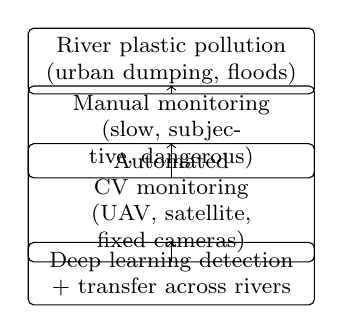
\begin{tikzpicture}[node distance=0.9cm, every node/.style={draw, rounded corners=2pt, text width=3.4cm, align=center, font=\footnotesize}]
\node (poll) {River plastic pollution\\(urban dumping, floods)};
\node (man) [below of=poll] {Manual monitoring\\(slow, subjective, dangerous)};
\node (auto) [below of=man] {Automated CV monitoring\\(UAV, satellite, fixed cameras)};
\node (dl) [below of=auto] {Deep learning detection\\+ transfer across rivers};
\draw[->] (poll) -- (man);
\draw[->] (man) -- (auto);
\draw[->] (auto) -- (dl);
\end{tikzpicture}
\caption{From river pollution evidence to automated monitoring: manual limits motivate continuous computer-vision observation, and deep learning must transfer across rivers to be useful.}
\label{fig:problem}
\end{figure}
